% article example for classicthesis.sty
\documentclass[10pt,a4paper]{article} % KOMA-Script article scrartcl
\usepackage{lipsum}
\usepackage{url}
\usepackage[nochapters]{classicthesis} % nochapters
\usepackage{polski}
\usepackage[utf8]{inputenc}
\usepackage{enumerate}
\usepackage{float}
\usepackage{subcaption}
\usepackage{graphicx}
\usepackage{amsmath}
\usepackage[T1]{fontenc}

\begin{document}
    \pagestyle{plain}
    \title{\rmfamily\normalfont\spacedallcaps{Opracowanie zagadnień na egzamin dyplomowy}}
    \date{} % no date

    \maketitle

    \tableofcontents

    \section{Zagadnienia obejmujące podstawowe treści programowe kierunku studiów Fizyka Techniczna do egzaminu dyplomowego na studiach II stopnia}
    \subsection{Ruch w mechanice newtonowskiej i relatywistycznej}
    
\begin{enumerate}[1]
\item \underline{Zasada dynamiki Newtona:}

I zasada dynamiki Newtona zakłada istnienie inercjalnego układu odniesienia. Układ inercjalny to taki, w którym cząstka nie podlegająca oddziaływaniu z otoczeniem, spoczywa lub porusza się po prostej ze stałą predkością (układy inercjalne poruszają się ruchem jednostajnym lub spoczywają względem siebie).

\item \underline{Zasada dynamiki Newtona:}
	
W inercjalnym układzie odniesienia jeśli siły działające na ciało nie rownoważą się ($ \vec{F_w} \neq 0 $) to ciało porusza się z przyśpieszeniem wprost proporcjonalnym do siły wypadkowej, a odwrotnie proporcjonalnym do masy ciała:\newline
$ \vec{a} = \frac{1}{m}*\vec{F_w} $\newline
$ \vec{F_w} = \frac{d\vec{p}}{dt} = \frac{d}{dt}(m\vec{v}) = m\frac{d\vec{v}}{dt} = m\vec{a} $\newline
Pierwsza zasada dynamiki Newtona jest szczególnym przypadkiem drugiej zasady dynamiki Newtona (gdy $ \vec{F_w} = 0 $).

\item \underline{Zasada dynamiki Newtona:}

Oddziaływania ciał są zawsze wzajemne. Jeżeli ciało \textit{A} działa na ciało \textit{B} siła $\vec{F}$ (akcja), to ciało \textit{B} działa na ciało \textit{A} siłą o takiej samej wartości i kierunku, lecz przeciwnym zwrocie (reakcja).
	
\end{enumerate}

\underline{Szczególna teoria względności}

\begin{enumerate}[1]
	\item \underline{postulat}:
	
We wszystkich układach inercjalnych prawa fizyki są jednakowe (zasada względności).

	\item \underline{postulat}:
	
Dla wszystkich obserwatorów inercjalnych prędkość światła w próżni (\textit{c}) jest taka sama i nie zależy od prędkości źródła światła.

\end{enumerate}

Te postualaty Einsteina prowadzą do tranformacji Lorentza:\newline
Rozważmy układ K oraz układ K' poruszający się względem K z predkością $ v_x $ wzdłuż osi OX (dla t = t' = 0 początki układów współrzednych $ 0_K $ i $ 0_{K'} $ pokrywają się), wtedy:\newline
$ t' = \gamma(\textit{t} - \frac{v_xx}{c^2}) $, $\gamma = \frac{1}{\sqrt{1-\frac{v_x^2}{c^2}}}$\newline
$ x'=\gamma(x - v_xt) $, y'=y, z'=z

Konsekwencje szczególnej teorii względności:

\begin{enumerate}[-]
\item Względność jednoczesności - dwa zdarzenia określone przez jednego obserwatora jako jednoczesne, mogą nie być jednoczesne dla innego obserwatora.
\item Dylatacja czasu - czas, jaki mija pomiędzy dwoma zdarzeniami, nie jest jednoznacznie określony, lecz zależy od ruchu obserwatora (paradoks bliźniąt).
\item Relatywistyczne składanie prędkości.
\item Masa jest równoważna energii $ E=mc^2 $.
\item Ciała bezmasowe poruszają się z prędkością c, dla ciał z niezerową masą niemożliwe jest osiągnięcie prędkości c.
\item Skrócenie Lorentza.
\end{enumerate}
    \subsection{Zasady zachowania i symetrie w fizyce}
	Jeśli układ posiada pewną symetrię, oznacza to, że równania opisujące ten układ nie zmieniają swojej postaci po dokonaniu przekształceń symetrii.

\underline{Dyskretne przekształcenia symetrii} to takie, których nie można sparametryzować np.
\begin{enumerate}[-]
	
\item Teoria grup i symetrii translacyjnej dla sieci periodycznej w kryształach.
\item Symetria permutacyjna funkcji falowej dla układu wielu ciał - związana z nierozróżnialnością cząstek elementarnych (zamiana miejscami cząstek układu nie zmiłaby równań opisujących układ).
\item Symetria zwierciadlana \textbf{P} związana z przekształceniem odbicia przestrzennego (zmiana znaków składowych przestrzennych wektorów na przeciwne).
\item Odwracalność w czasie \textbf{T} (zmiana znaku czasu w równaniach).
\item Parzystość ładunkowa \textbf{C} (zmiana znaku ładunku).

\end{enumerate}

Elektromagnetyzm, grawitacja i oddziaływania silne są niezmiennicze względem każdej z ostatnich trzech wymienionych symetrii (CPT) osobno, jednakże w przypadku oddziaływań słabych niezmienniczość jest zachowana tylko w przypadku łącznego ich działania CPT (rozpad $ \beta $ łamie symetrie P i C, ale zachowuje połączoną symetrie CP, która dla odmiany jest łamana w przypadku rozpadu mezonów K).

\underline{Symetrie związane z ciągłymi przekształceniami} są bezpośrednio związane z istnieniem zasad zachowania - związek ten opisuje twierdzenie Noether. Zgodnie z tym twierdzeniem, z daną symetrią układu jest związanych tyle praw zachowania, ile ciągłych rzeczywistych parametrów potrzebnych jest do sparametryzowania odpowiadających tej symetrii przekształceń np.

\begin{enumerate}[-]
\item Zasada zachowania energii wynika z symetrii związanej z przesunięciem w czasie - niezmienniczości działania S opisującego ruch danego układu od czasu (t - parametr). Jeżeli układ absorbuje lub emituje energie, wówcząs to działanie jest funkcją czasu (t) - odpowiada to w konsekwencji zmianie energii układu.

\item Zasada zachowania pędu wynika z symetrii związanej z przesunięciem układu w przestrzeni.

\item Zasada zachowania momentu pędu wynika z z symetrii związanej z obrotem układu.

\item Zasada zachowania ładunku wyniki z niezmienniczości funkcji falowej elektronu względem transformacji cechowania.
\end{enumerate}
	\subsection{Klasyczny i kwantowy oscylator harmoniczny}
	Lalala
	\subsection{Fizyczna treść równań Maxwella i równania falowego.}
	\begin{figure} [H]
	\centering
	\begin{subfigure}{.49\textwidth}
		\centering
		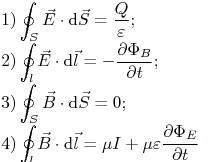
\includegraphics[width=1.0\linewidth]{generalIssues/Figures/maxwell1.png}
		\caption{Postać całkowa.}
		\label{n1}
	\end{subfigure}
	\begin{subfigure}{.49\textwidth}
		\centering
		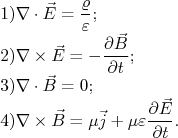
\includegraphics[width=1.0\linewidth]{generalIssues/Figures/maxwell2.png}
		\caption{Postać różniczkowa.}
		\label{r1}
	\end{subfigure}
	\caption{Równania Maxwella.}
	\label{maxwell}
\end{figure}

Rysunek~\ref{maxwell} przedstawia równania Maxwella, gdzie:\newline
$ \varrho $ - gęstość ładunku,\newline
$ \varepsilon $ - przenikalność dielektryczna,\newline
$ \mu $ - przenikalność magnetyczna,\newline
$ \vec{j} $ - gęstość prądu,\newline
$ \Phi_B $- strumień indukcji magnetycznej,\newline
$ \Phi_E $- strumień natężenia pola elektrycznego,\newline
$ \nabla * \vec{F} = \frac{\partial F_x(x,y,z)}{\partial x} + \frac{\partial F_y(x,y,z)}{\partial y} + \frac{\partial F_z(x,y,z)}{\partial z}$ - dywergencja pola wektorowego $ \vec{F} = [F_x, F_y, F_z] $,\newline
$
\nabla \times \vec{F} = 
\begin{vmatrix}
\textbf{i} & \textbf{j} & \textbf{k} \\ 
\frac{\partial}{\partial x} & \frac{\partial}{\partial y} & \frac{\partial}{\partial z} \\ 
F_x & F_y & F_z  \notag
\end{vmatrix}
= (\frac{\partial F_z}{\partial y} - \frac{\partial F_y}{\partial z})\textbf{i} + (\frac{\partial F_x}{\partial z} - \frac{\partial F_z}{\partial x})\textbf{j} + (\frac{\partial F_y}{\partial x} - \frac{\partial F_x}{\partial y})\textbf{k}
$ - rotacja pola wektorowego $ \vec{F} $.\newline

Sens fizyczny praw Maxwella:
\begin{enumerate}[1)]
	\item \underline{Prawo Gaussa dla elektryczności} - źródłem pola elektrycznego są ładunki, a strumień tego pola przez dowolną powierzchnię zamkniętą zależy tylko od ładunku zamkniętego przez tę powierzchnię.
	\item \underline{Prawo Faradaya} - zmiana strumienia indukcji magnetycznej przez powierzchnię zamkniętej pętli powoduje powstanie w tej pętli siły elektromotorycznej indukcji (SEM), a kierunek płynącego prądu jest taki, żeby przeciwdziałać zmianom powodującym indukcję (reguła Lenza).
	\item \underline{Prawo Gaussa dla magnetyzmu} - nie istnieją ładunki magnetyczne, a strumień pola magnetycznego przez dowolną powierzchnię zamkniętą jest równy 0.
	\item \underline{Prawo Ampere'a} - zmienne pole elektryczne i płynący prąd powodują powstanie pola magnetycznego.
\end{enumerate}

Dla fali elektromagnetycznej w próżni wektory $ \vec{E} $ i $ \vec{B} $ drgają w płaszczyznach wzajemnie prostopadłych i dla fali rozchodzącej się w kierunku osi x możemy przyjąć taki układ odniesienia aby wektor $ \vec{E} $ drgał w kierunku osi y a wektor $ \vec{B} $ w kierunku osi z. Zatem wektory $ \vec{E} $ i $ \vec{B} $ mają tylko po jednej składowej:\newline
$ \vec{E} = [0, E, 0] $,\newline
$ \vec{B} = [0, 0, B] $.\newline
Liczmy rotację wektorów $ \vec{E} $ i $ \vec{B} $ (wykorzystując fakt, że nasza fala jest falą płaską i pola $ \vec{E} $ i $ \vec{B} $ zmieniają się tylko względem współrzędnej x, czyli że $ \frac{\partial E}{\partial z} = 0, \frac{\partial B}{\partial y} = 0$):\newline
$ \nabla \times \vec{E} = \textbf{k}\frac{\partial E}{\partial x} $,\newline
$ \nabla \times \vec{B} = -\textbf{j}\frac{\partial B}{\partial x} $.\newline

Korzystając z równań Faradaya oraz Ampera w postaci różniczkowej otrzymujemy (poszukujemy równania dla fal elektromagnetycznych rozchodzących się w próżni gdzie nie będą występowały prądy przewodzenia, czyli $ \vec{j} $ = 0):\newline
$ \textbf{k}\frac{\partial E}{\partial x} = -\frac{\partial \vec{B}}{\partial t} = -\textbf{k}\frac{\partial B}{\partial t} $,\newline
$ \textbf{j}\frac{\partial B}{\partial x} = -\mu_0 \epsilon_0 \frac{\partial \vec{E}}{\partial t} = -\textbf{j} \mu_0 \epsilon_0 \frac{\partial E}{\partial t} $.\newline
W efekcie dostajemy układ dwóch równań:\newline
$ \frac{\partial E}{\partial x} = -\frac{\partial B}{\partial t} $,\newline
$ \frac{\partial B}{\partial x} = - \mu_0 \epsilon_0 \frac{\partial E}{\partial t} $.\newline

Równania falowe dla $ \vec{E} $ i $ \vec{B} $ będą miały identyczną postać. Jeżeli zdecydujemy się szukać równania dla $ \vec{E} $, to eliminujemy z naszego układu równań $ \vec{B} $ przez utworzenie pochodnych mieszanych $ \vec{E} $ względem x i t. Różniczkujemy zatem pierwsze równanie po x, a drugie po t (jeśli chcemy szukać równania dla $ \vec{B} $ eliminujemy w ten sam sposób z naszych równań $ \vec{E} $):\newline
$ \frac{\partial^2 E}{\partial x^2} = -\frac{\partial^2 B}{\partial t \partial x} $,\newline
$ \frac{\partial^2 B}{\partial t \partial x} = - \mu_0 \epsilon_0 \frac{\partial^2 E}{\partial t^2} $.\newline
Z powyższego układu równań otrzymujemy poszukiwane równanie falowe dla pola $ \vec{E} $:\newline
$ \frac{\partial^2 E}{\partial x^2} - \mu_0 \epsilon_0 \frac{\partial^2 E}{\partial t^2} = 0 $\newline
Znając ogólną postać równania falowego dla fali rozchodzącej się z predkością v w kierunku osi x:\newline
$ \frac{\partial^2 \xi}{\partial x^2} - \frac{1}{v^2} \frac{\partial^2 \xi}{\partial t^2} = 0 $\newline
otrzymujemy związek pomiędzy prędkością światła w próżni (c) a wartościami przenikalności elektrycznej i magnetycznej próżni: \newline
$ c = \frac{1}{\sqrt{\mu_0 \epsilon_0}} $.\newline
Rozwiązanie równania falowego dla pola $ \vec{E} $ ma postać:\newline
$ \vec{E} = \vec{E_0}\sin(kx - \omega t) $,\newline
gdzie: $ k = \frac{2\pi}{\lambda} $, $ \omega = ck $.
	
    \section{Specjalność: Eksploracja Danych i Modelowanie Interdyscyplinarne}

\end{document}
